%****************************************************************************%
%* JFTP Module                                                              *%
%*                                                                          *%
%* Author(s):                                                               *%
%* - Abdelkader AMAR (Abdelkader.Amar@ens-lyon.fr)                          *%
%* - David LOUREIRO (David.Loureiro@ens-lyon.fr)                            *%
%*                                                                          *%
%* $LICENSE$                                                                *%
%****************************************************************************%
%* $Id: GUM_JFTP.tex,v 1.5 2007/11/29 16:03:21 dloureir Exp $
%* $Log: GUM_JFTP.tex,v $
%* Revision 1.5  2007/11/29 16:03:21  dloureir
%* typo corrections
%*
%* Revision 1.4  2007/11/29 10:49:23  dloureir
%* Correcting the wrong caption text
%*
%* Revision 1.3  2007/11/08 16:53:48  dloureir
%* Adding the ganglia part in the User's Manual
%*
%* Revision 1.2  2007/11/08 11:31:14  dloureir
%* Correcting the headers
%*
%****************************************************************************%
\chapter{JFTP Module for \grudu}
\section{Presentation}
JFTP is an acronym for \textit{\textbf{J}ava \textbf{F}ile \textbf{T}ransfert
\textbf{P}rotocol}. JFTP is a graphical Java network and file transfer client.
At the origin JFTP is developed as a project under GNU GPL license. You can find
more information about the initial project at
\url{http://j-ftp.sourceforge.net/}. 

JFTP has been modify to corresponds to the needs of the GRUDU users. Thanks to
the modified JFTP you can transfer data between you local machine and \gfk, but
also between \gfk frontales.

\section{Interface}

The JFTP module presents three internal frames, one for the local machine, one
for \gfk with one tab per site, and the last frame for the log of the module.

\begin{figure}[H]
	\centering
	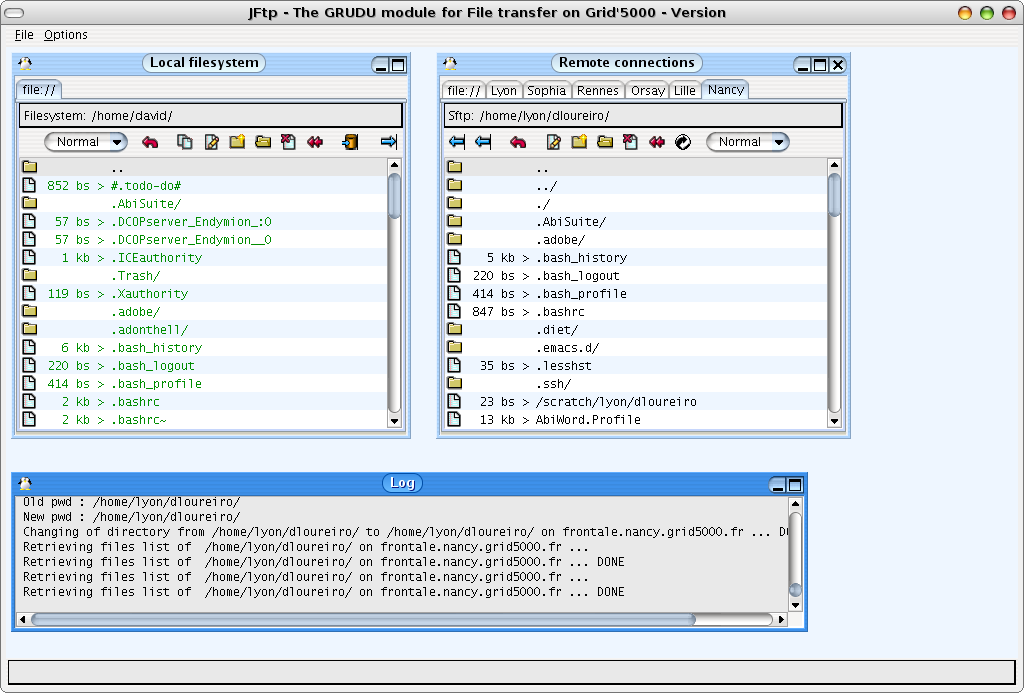
\includegraphics[width=0.7\linewidth]{figures/GRUDU_jftp1.eps}
	\caption{JFTP main interface}
	\label{fig:GRUDU_jftp1}
\end{figure}

For the configuration of the options for the Rsync transfert between \gfk
frontales, you can click on the option menu and you will find the following
frame where you can edit the Rsync options:

\begin{figure}[H]
	\centering
	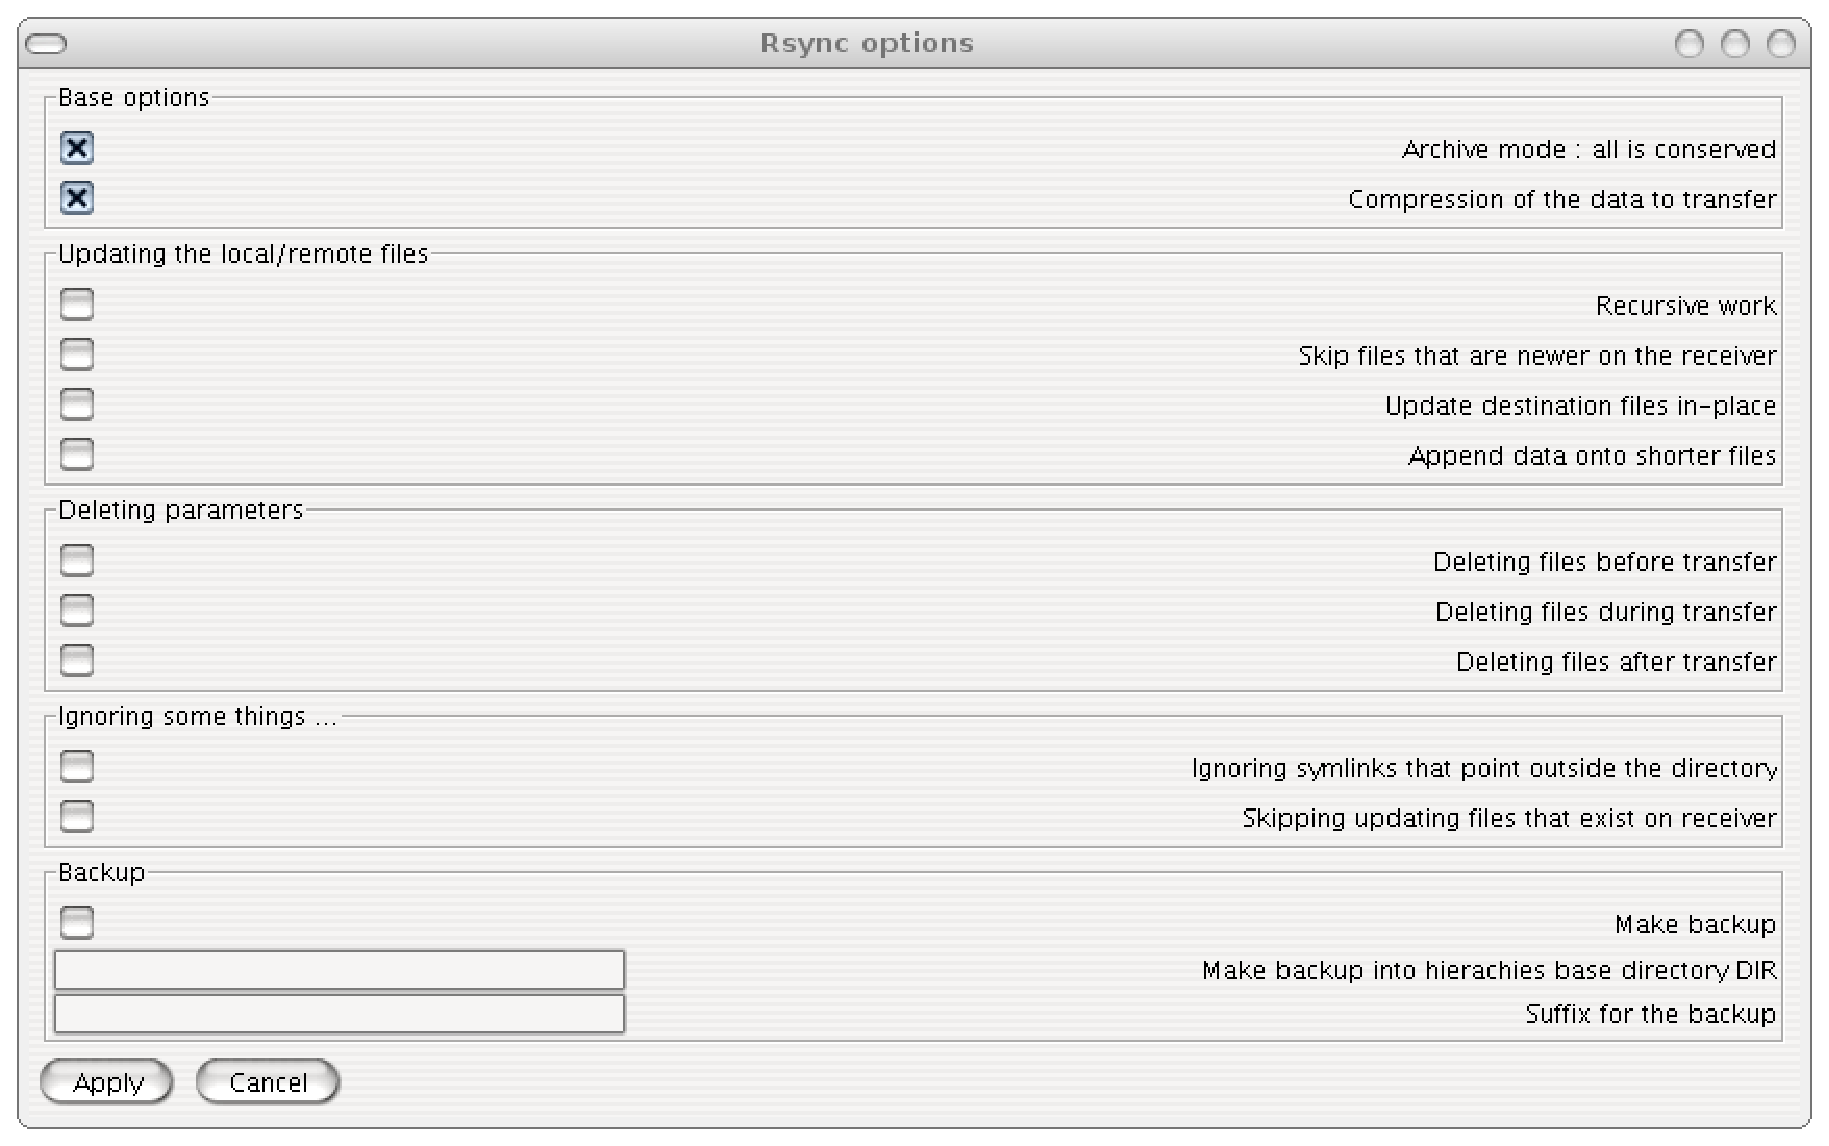
\includegraphics[width=0.5\linewidth]{figures/GRUDU_jftp2.eps}
	\caption{JFTP rsync options}
	\label{fig:GRUDU_jftp2}
\end{figure}

%******************************************%